\documentclass{beamer}

\usepackage[utf8]{inputenc}
\usepackage[T1]{fontenc}
\usepackage{tikz}
\usepackage{siunitx}
\usepackage{pgfplots}
\usepackage{listings}

\usetheme{Copenhagen}

\title{Physically based rendering}
\subtitle{Progressive photon mapping}
\author[Bannier, Helali, Louarn]{Kévin \textsc{Bannier} \and Billel \textsc{Hélali} \and Amaury \textsc{Louarn}}
\institute{\'Ecole Supérieure d'ingénieurs de Rennes\\Université de Rennes 1}
\logo{\def\svgwidth{2cm}\input{esir.pdf_tex}}

\usepgfplotslibrary{units}

\AtBeginSection[]
{
       \begin{frame}
           \frametitle{Table of contents}
           \tableofcontents[currentsection]
      \end{frame}
}

\begin{document}
\frame{\titlepage}

\section{What is progressive photon mapping?}
\begin{frame}
    \frametitle{Definition}
    \begin{itemize}
        \item Photon mapping belongs to the family of the particle-tracing algorithms
        \item Constructing paths from the light onto the objects
            \vfill
        \item 2 stages:
            \begin{enumerate}
                \item Generating and sending the photons, with arbitrary accuracy and without storing the full photon map
                \item Final gathering
            \end{enumerate}
        \item Repeat this principle several times and calculate the average picture
    \end{itemize}
\end{frame}
\begin{frame}
    \frametitle{Algorithm}
    \tt
    \begin{itemize}
        \item nbIterations = 10000;
        \item nbPhotons = 250000;
        \item calculateAllIntersectionsWithScene();
        \item for i = 0 to nbIterations:
            \begin{itemize}
                \item sendPhotons();
                \item gatherPhotons();
                \item meanRenders();
            \end{itemize}
    \end{itemize}
\end{frame}

\begin{frame}
    \frametitle{More precisely}
    \begin{figure}
        \centering
        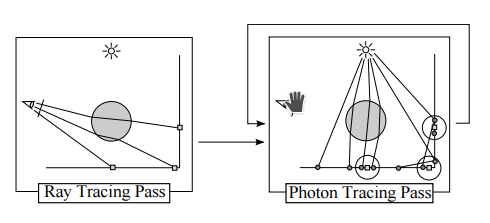
\includegraphics[height=2cm]{img/PPM}
    \end{figure}
    Multi-pass algorithm:
    \begin{enumerate}
        \item Ray tracing pass
            \begin{itemize}
                \item ray tracing to find all the visible surfaces
            \end{itemize}
        \item Photon tracing passes
            \begin{itemize}
                \item Every photon tracing increases the solution
                \item Convergence to an optimal solution in infinite time
            \end{itemize}
    \end{enumerate}
\end{frame}

\section{Criteria of comparison}
\begin{frame}
    \frametitle{Criteria of comparison}
    Several parameters for the progressive photon mapper:
    \begin{description}
        \item[Photons per iteration:] The number of photons to be sent at each iteration
        \item[Maximum depth:] The maximum depth of the final gathering rays
        \item[Russian roulette starting depth:] The depth before starting to eliminate photons with the russian roulette algorithm
        \item[Initial radius:] Initial photon query radius
    \end{description}
\end{frame}
\begin{frame}
    \frametitle{Photons per iteration}
    \begin{minipage}{0.5\textwidth}
    \end{minipage}
    \begin{minipage}{\textwidth}
        \begin{figure}
            \centering
            \begin{tikzpicture}[scale=0.6]
                \begin{axis}[
                    ]
                    \addplot
                    table[x=Photons per iteration, y=PSNR, col sep=comma] {data/photons.csv};
                \end{axis}
            \end{tikzpicture}
            \caption{PSNR according to the number of photons per iteration}
        \end{figure}
    \end{minipage}
\end{frame}
\begin{frame}
    \begin{figure}
        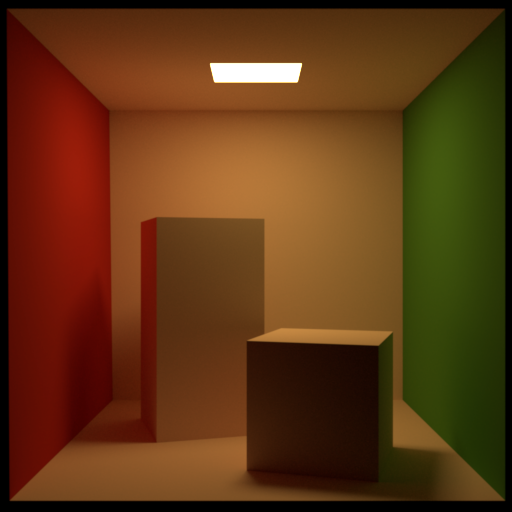
\includegraphics[width=0.5\textwidth]{img/params/cbox}
        \caption{Rendu parfait}
    \end{figure}
\end{frame}
\begin{frame}
    \begin{figure}
        \includegraphics[width=0.5\textwidth]{img/params/photons}
        \caption{500 000 photons per iteration}
    \end{figure}
\end{frame}
\begin{frame}
    \frametitle{Maximum depth}
    %\begin{minipage}{0.4\textwidth}
    %    \begin{figure}
    %        \includegraphics[width=0.5\textwidth]{img/params/depth}
    %        \caption{Max depth = 10}
    %    \end{figure}
    %\end{minipage}

    \begin{minipage}{\textwidth}
        \begin{figure}
            \centering
            \begin{tikzpicture}[scale=0.6]
                \begin{axis}[
                    ]
                    \addplot
                    table[x=Maximum depth, y=PSNR, col sep=comma] {data/depth.csv};
                \end{axis}
            \end{tikzpicture}
            \caption{PSNR according to the maximum depth}
        \end{figure}
    \end{minipage}
\end{frame}
\begin{frame}
    \begin{figure}
        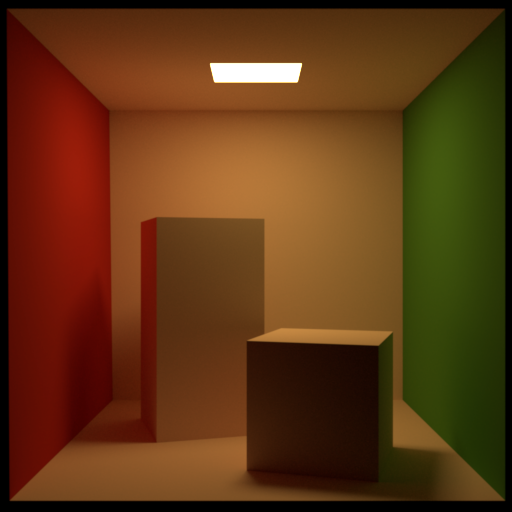
\includegraphics[width=0.5\textwidth]{img/params/cbox}
        \caption{Rendu parfait}
    \end{figure}
\end{frame}
\begin{frame}
    \begin{figure}
        \includegraphics[width=0.5\textwidth]{img/params/depth}
        \caption{Max depth = 10}
    \end{figure}
\end{frame}
\begin{frame}
    \frametitle{Initial radius}
    \begin{minipage}{0.5\textwidth}
    \end{minipage}
    \begin{minipage}{\textwidth}
        \begin{figure}
            \centering
            \begin{tikzpicture}[scale=0.6]
                \begin{axis}[
                    ]
                    \addplot
                    table[x=Initial radius, y=PSNR, col sep=comma] {data/initRadius.csv};
                \end{axis}
            \end{tikzpicture}
            \caption{PSNR according to the initial radius}
        \end{figure}
    \end{minipage}
\end{frame}
\begin{frame}
    \begin{figure}
        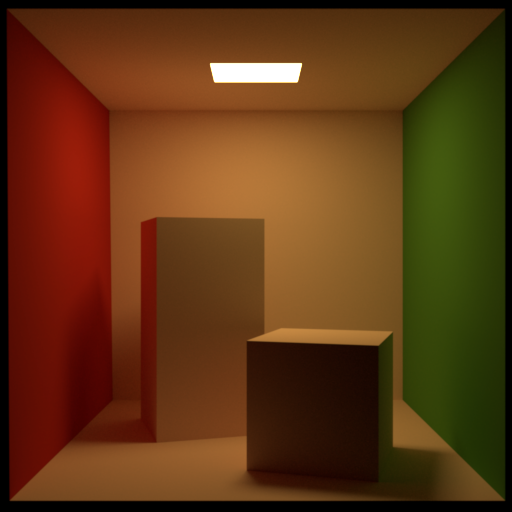
\includegraphics[width=0.5\textwidth]{img/params/cbox}
        \caption{Rendu parfait}
    \end{figure}
\end{frame}
\begin{frame}
    \begin{figure}
        \includegraphics[width=0.5\textwidth]{img/params/radius}
        \caption{Initial based on scene}
    \end{figure}
\end{frame}
\begin{frame}
    \frametitle{Russian roulette starting depth}
    \begin{minipage}{0.5\textwidth}
    \end{minipage}
    \begin{minipage}{\textwidth}
        \begin{figure}
            \centering
            \begin{tikzpicture}[scale=0.6]
                \begin{axis}[
                    ]
                    \addplot
                    table[x=Russian roulette start depth, y=PSNR, col sep=comma] {data/RR.csv};
                \end{axis}
            \end{tikzpicture}
            \caption{PSNR according to the russian roulette starting depth}
        \end{figure}
    \end{minipage}
\end{frame}
\begin{frame}
    \begin{figure}
        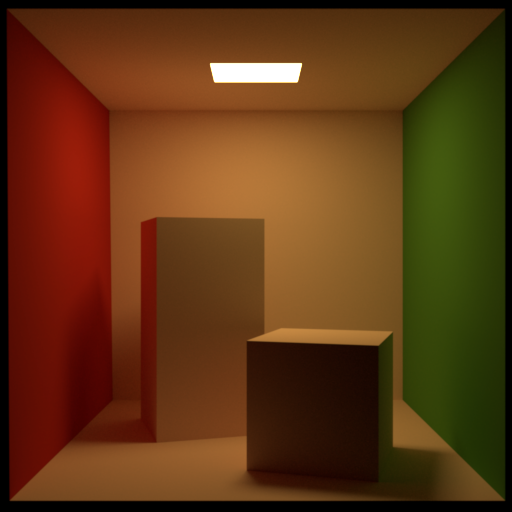
\includegraphics[width=0.5\textwidth]{img/params/cbox}
        \caption{Rendu parfait}
    \end{figure}
\end{frame}
\begin{frame}
    \begin{figure}
        \includegraphics[width=0.5\textwidth]{img/params/RR}
        \caption{Russian Roulette based on scene}
    \end{figure}
\end{frame}

\section{Results}
\begin{frame}
    \frametitle{Context}
    \begin{itemize}
        \item Image rendering for the cinema (e.g special effects)
        \item Time-constrained rendering (each render must not take more than a specified amount of time)
        \item Possiblity of a render farm: the method must be scalable
            \vfill
        \item Signal-perfect images are not necessary:
            \begin{itemize}
                \item Each image will not be on the screen for more than $1/24$th of a second
                \item (Often) presence of motion blur
            \end{itemize}
    \end{itemize}
\end{frame}

\begin{frame}
    \frametitle{Scalability}
    \begin{figure}
        \centering
        \begin{tikzpicture}
            \begin{axis}[
                    scale=0.8,
                    xlabel=cores,
                    ylabel=SSIM,
                    y unit=\%,
                    legend pos=outer north east
                ]
                \addplot[color=red, mark=x] table[x=cores, y=SSIM R,  col sep=comma]{data/cores.csv};
                \addplot[color=green, mark=x] table[x=cores, y=SSIM G,  col sep=comma]{data/cores.csv};
                \addplot[color=blue, mark=x] table[x=cores, y=SSIM B,  col sep=comma]{data/cores.csv};
                \legend{SSIM R, SSIM G, SSIM B}
            \end{axis}
        \end{tikzpicture}
    \end{figure}
\end{frame}

\begin{frame}
    \frametitle{Time-constrained rendering}
    \begin{figure}
        \centering
        \begin{tikzpicture}
            \begin{axis}[
                    scale=0.8,
                    xlabel=time,
                    ylabel=SSIM,
                    x unit=min,
                    y unit=\%,
                    legend pos=outer north east
                ]
                \addplot[color=red] table[x=temps_mn, y=SSIM R, col sep=comma] {data/SLS.csv};
                \addplot[color=green] table[x=temps_mn, y=SSIM G, col sep=comma] {data/SLS.csv};
                \addplot[color=blue] table[x=temps_mn, y=SSIM B, col sep=comma] {data/SLS.csv};
                \addplot[color=gray] table[x=temps_mn, y=mean SSIM, col sep=comma] {data/SLS.csv};
                \legend{SSIM R, SSIM G, SSIM B, mean SSIM}
            \end{axis}
        \end{tikzpicture}
    \end{figure}
\end{frame}

\begin{frame}
    \frametitle{Render process (1/4)}
    \begin{figure}
        \centering
        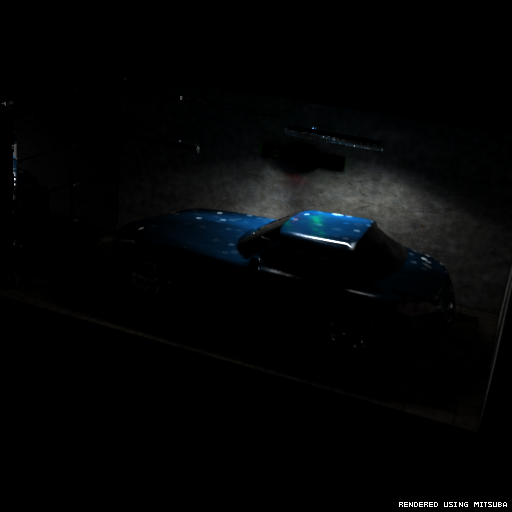
\includegraphics[width=0.6\textwidth]{img/SLS/1.png}
    \end{figure}
\end{frame}
\begin{frame}
    \frametitle{Render process (2/4)}
    \begin{figure}
        \centering
        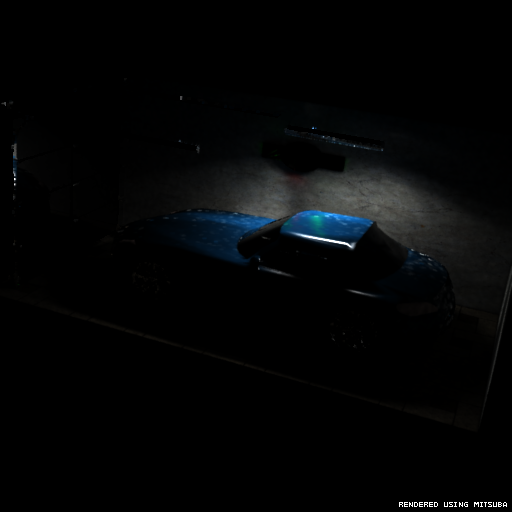
\includegraphics[width=0.6\textwidth]{img/SLS/2.png}
    \end{figure}
\end{frame}
\begin{frame}
    \frametitle{Render process (3/4)}
    \begin{figure}
        \centering
        \includegraphics[width=0.6\textwidth]{img/SLS/3.png}
    \end{figure}
\end{frame}
\begin{frame}
    \frametitle{Render process (4/4)}
    \begin{figure}
        \centering
        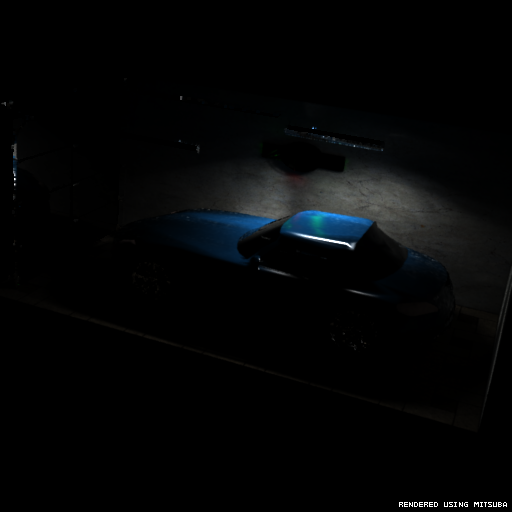
\includegraphics[width=0.6\textwidth]{img/SLS/4.png}
    \end{figure}
\end{frame}

\end{document}
